\begin{anexosenv}
	
	% Imprime uma página indicando o início dos anexos
	\partanexos
	
	% ---
	\chapter{Requisitos funcionais}
	% ---
	
	\begin{table}[htbp]
\centering
\caption{Requisito de identificação de acesso dos usuários.}
\label{tab:rf01}
\begin{tabular}{l p{10cm}}
\toprule
\multicolumn{2}{c}{RF01 - IDENTIFICADOR DE ACESSO} \\ \midrule
Descrição:  & O sistema deverá ser capaz de identificar o usuário local.  \\ \midrule
Prioridade: & [ x ] Essencial    [   ] Importante    [   ] Desejável \\ \bottomrule
\end{tabular}
\end{table}


\begin{table}[htbp]
\centering
\caption{Requisito para cadastrar produtos.}
\label{tab:rf02}
\begin{tabular}{l p{10cm}}
\toprule
\multicolumn{2}{c}{RF02 - CADASTRAR PRODUTOS} \\ \midrule
Descrição:  & O sistema deverá permitir o cadastro de novos produtos podendo armazenar o maior número de informações disponíveis.\\ \midrule
Prioridade: & [ x ] Essencial    [   ] Importante    [   ] Desejável \\ \bottomrule
\end{tabular}
\end{table}

\begin{table}[htbp]
\centering
\caption{Requisito para editar produtos.}
\label{tab:rf03}
\begin{tabular}{l p{10cm}}
\toprule
\multicolumn{2}{c}{RF03 - EDITAR PRODUTOS} \\ \midrule
Descrição:  & O sistema deve permitir editar as informações de um produto cadastrado.\\ \midrule
Prioridade: & [   ] Essencial    [ x ] Importante    [   ] Desejável \\ \bottomrule
\end{tabular}
\end{table}

\begin{table}[htbp]
\centering
\caption{Requisito para excluir produtos.}
\label{tab:rf04}
\begin{tabular}{l p{10cm}}
\toprule
\multicolumn{2}{c}{RF04 - EXCLUIR PRODUTOS} \\ \midrule
Descrição:  & O sistema deve permitir excluir um produto cadastrado.\\ \midrule
Prioridade: & [   ] Essencial    [ x ] Importante    [   ] Desejável \\ \bottomrule
\end{tabular}
\end{table}

\begin{table}[H]
\centering
\caption{Requisito para consultar produtos.}
\label{tab:rf05}
\begin{tabular}{l p{10cm}}
\toprule
\multicolumn{2}{c}{RF05 - CONSULTAR PRODUTOS} \\ \midrule
Descrição:  & O sistema deve realizar uma consulta por um produto cadastrado.\\ \midrule
Prioridade: & [   ] Essencial    [ x ] Importante    [   ] Desejável \\ \bottomrule
\end{tabular}
\end{table}

\begin{table}[htbp]
\centering
\caption{Requisito para cadastrar clientes.}
\label{tab:rf06}
\begin{tabular}{l p{10cm}}
\toprule
\multicolumn{2}{c}{RF06 - CADASTRAR CLIENTES} \\ \midrule
Descrição:  & O sistema deverá permitir o cadastro de novos clientes podendo armazenar o maior número de informações sobre o cliente.\\ \midrule
Prioridade: & [ x ] Essencial    [   ] Importante    [   ] Desejável \\ \bottomrule
\end{tabular}
\end{table}

\begin{table}[htbp]
\centering
\caption{Requisito para editar clientes.}
\label{tab:rf07}
\begin{tabular}{l p{10cm}}
\toprule
\multicolumn{2}{c}{RF07 - EDITAR CLIENTES} \\ \midrule
Descrição:  & O sistema deve permitir editar as informações de um cliente cadastrado.\\ \midrule
Prioridade: & [   ] Essencial    [ x ] Importante    [   ] Desejável \\ \bottomrule
\end{tabular}
\end{table}

\begin{table}[htbp]
\centering
\caption{Requisito para excluir produtos.}
\label{tab:rf08}
\begin{tabular}{l p{10cm}}
\toprule
\multicolumn{2}{c}{RF08 - EXCLUIR CLIENTE} \\ \midrule
Descrição:  & O sistema deve permitir excluir um cliente cadastrado.\\ \midrule
Prioridade: & [   ] Essencial    [ x ] Importante    [   ] Desejável \\ \bottomrule
\end{tabular}
\end{table}

\begin{table}[htbp]
\centering
\caption{Requisito para consultar clientes.}
\label{tab:rf09}
\begin{tabular}{l p{10cm}}
\toprule
\multicolumn{2}{c}{RF09 - CONSULTAR CLIENTES} \\ \midrule
Descrição:  & O sistema deve realizar uma consulta de um cliente cadastrado.\\ \midrule
Prioridade: & [   ] Essencial    [ x ] Importante    [   ] Desejável \\ \bottomrule
\end{tabular}
\end{table}

\begin{table}[htbp]
	\centering
	\caption{Requisito para gerar orçamentos.}
	\label{tab:rf18}
	\begin{tabular}{l p{10cm}}
		\toprule
		\multicolumn{2}{c}{RF18 - GERAR ORÇAMENTOS} \\ \midrule
		Descrição:  & O sistema deverá gerar orçamentos detalhados com base no estoque da empresa e de clientes cadastrados \\ \midrule
		Prioridade: & [ x ] Essencial    [   ] Importante    [   ] Desejável \\ \bottomrule
	\end{tabular}
\end{table}

\begin{table}[htbp]
	\centering
	\caption{Requisito de alerta de estoque.}
	\label{tab:rf19}
	\begin{tabular}{l p{10cm}}
		\toprule
		\multicolumn{2}{c}{RF19 - ALERTA DE ESTOQUE} \\ \midrule
		Descrição:  & O sistema deverá emitir alertas quando um produto estiver em quantidade abaixo do nível ideal no estoque.\\ \midrule
		Prioridade: & [ x ] Essencial    [   ] Importante    [   ] Desejável \\ \bottomrule
	\end{tabular}
\end{table}
	
	% ---
\chapter{Requisitos Não-funcionais}

\begin{table}[htbp]
	\centering
	\caption{Restrição de acesso ao banco de dados.}
	\label{tab:rnf01}
	\begin{tabular}{l p{10cm}}
		\toprule
		\multicolumn{2}{c}{RNF01 - RESTRIÇÃO DE ACESSO AO BANCO DE DADOS} \\ \midrule
		Categoria:  & Segurança\\ \midrule
		Descrição:  & O acesso ao banco de dados deve ser protegido e restrito a somente usuários devidamente autorizados.\\ \midrule
		Prioridade: & [ x ] Essencial    [   ] Importante    [   ] Desejável \\ \bottomrule
	\end{tabular}
\end{table}

\begin{table}[htbp]
	\centering
	\caption{Linguagem de programação do sistema.}
	\label{tab:rnf02}
	\begin{tabular}{l p{10cm}}
		\toprule
		\multicolumn{2}{c}{RNF02 - LINGUAGEM DE PROGRAMAÇÃO} \\ \midrule
		Categoria:  & Compatibilidade\\ \midrule
		Descrição:  & O sistema deverá ser desenvolvido em linguagem JAVA.\\ \midrule
		Prioridade: & [   ] Essencial    [ x ] Importante    [   ] Desejável \\ \bottomrule
	\end{tabular}
\end{table}

\begin{table}[htbp]
	\centering
	\caption{Interface gráfica do sistema.}
	\label{tab:rnf03}
	\begin{tabular}{l p{10cm}}
		\toprule
		\multicolumn{2}{c}{RNF03 - INTERFACE GRÁFICA} \\ \midrule
		Categoria:  & Usabilidade\\ \midrule
		Descrição:  & O sistema deverá possuir uma interface amigável, intuitiva e de fácil manipulação.\\ \midrule
		Prioridade: & [ x ] Essencial    [   ] Importante    [   ] Desejável \\ \bottomrule
	\end{tabular}
\end{table}

\begin{table}[htbp]
	\centering
	\caption{Validação de dados}
	\label{tab:rnf04}
	\begin{tabular}{l p{10cm}}
		\toprule
		\multicolumn{2}{c}{RNF04 - VALIDAÇÃO DE DADOS} \\ \midrule
		Categoria:  & Confiabilidade\\ \midrule
		Descrição:  & O sistema deverá validar os dados que serão armazenados no banco de dados afim de evitar dados repetidos ou inválidos.\\ \midrule
		Prioridade: & [ x ] Essencial    [   ] Importante    [   ] Desejável \\ \bottomrule
	\end{tabular}
\end{table}

%\begin{table}[htbp]
%	\centering
%	\caption{Disponibilidade das informações.}
%	\label{tab:rnf05}
%	\begin{tabular}{l p{10cm}}
%		\toprule
%		\multicolumn{2}{c}{RNF05 - DISPONIBILIDADE DAS INFORMAÇÕES} \\ \midrule
%		Categoria:  & Disponibilidade\\ \midrule
%		Descrição:  & Os dados armazenado devem estar disponíveis aos usuários %sempre que solicitado\\ \midrule
%		Prioridade: & [ x ] Essencial    [   ] Importante    [   ] Desejável \\ %\bottomrule
%	\end{tabular}
%\end{table}

\chapter{Diagramas de classes}

\begin{figure}[htp]
\centering
\caption{Diagrama de classes}
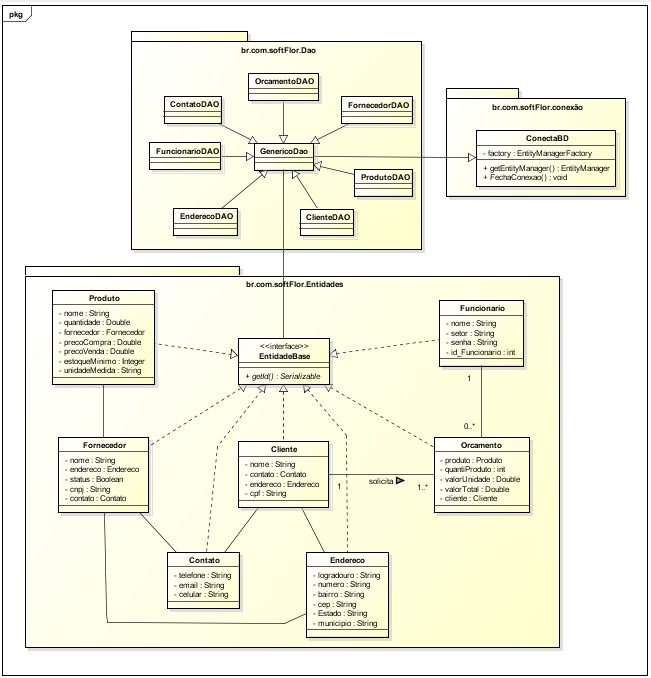
\includegraphics[width=18cm]{imagens/diagramas/DiagramaClasses}
\fonte{Autor próprio}
\label{fig:Diagrama de classes}
\end{figure}

	
\chapter{Diagramas de atividade}

	
\chapter{Diagramas de sequência}


\chapter{Diagrama Modelo entidade-Relacionamento}

\begin{figure}[H]
\centering
\caption{Diagrama MER}
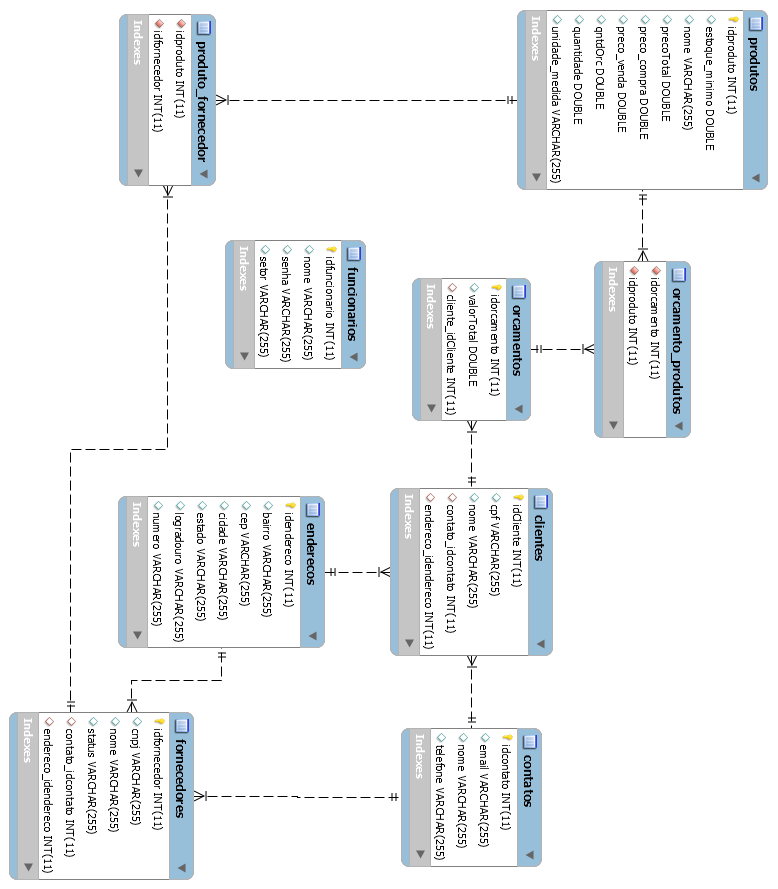
\includegraphics[width=17cm]{imagens/diagramas/bd}
\fonte{Autor próprio}
\label{fig:Diagrama MER}
\end{figure}

\chapter{Código Java e Código do Banco de dados}
	% ---
	Todo os códigos deste sistema esta disponível na plataforma de hospedagem de código-fonte GitHub e pode ser acessado através da URL: https://github.com/loardjulio/SoftFlor.git
	
\end{anexosenv}